\chapter{Risultati}%Caratterizzazione DDS su HPC
% Visti i diversi risultati si può dire che è meglio usare i topic per* le partizioni per *
% etc etc

Nella sezione corrente, si riportano tutti i risultati rilevanti ottenuti durante la fase di testing e verrà stilato un modello di use-case utile alle finalità di Power Management.

\section{Impatto del numero di sub in un dominio}
Visto lo schema \ref{fig:uml} risulta facile capire, che il numero di subscriber presenti in un dominio comporta un overhead di comunicazione che va ad influenzare sia i tempi, che i cicli, che le istruzioni impiegate nella singola \emph{publish} su un topic come viene facilmente dimostrato nella figura\ref{fig:test3_overhead}.
\begin{figure}[H]
    \centering
    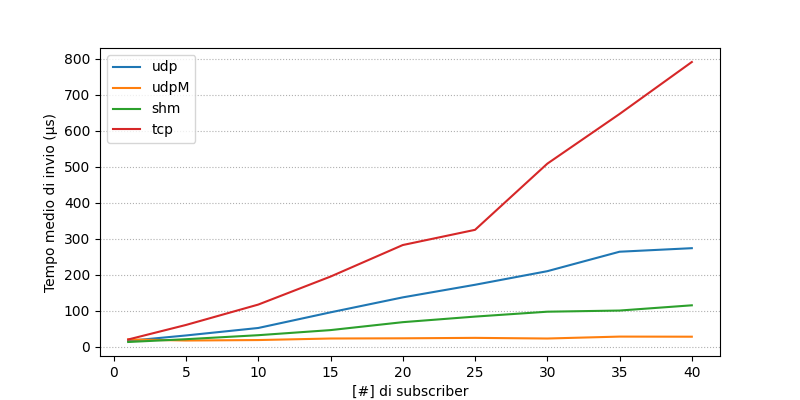
\includegraphics[width=\textwidth]{./results/test3_sending_multiplesub.png} %TODO, sqeunce is an error
    \caption{overhead sulla publish all'aumentare dei subscriber}
    \label{fig:test3_overhead}
\end{figure}
\begin{figure}[H]
    \centering
    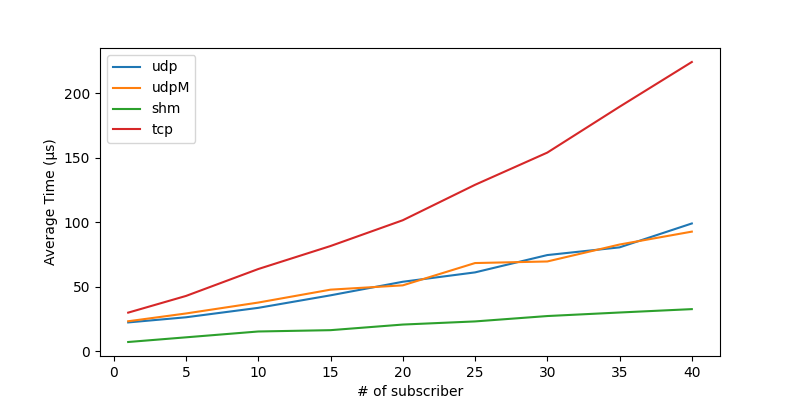
\includegraphics[width=\textwidth]{./results/test3_sendingreceiving_multiplesub.png} 
    \caption{latenza di ricezione all'aumentare dei subscriber}
    \label{fig:test3_overhead}
\end{figure}

Ovviamente l'impatto è poco significativo in quei protocolli che applicano strutture di \gls{multicasting} come udp-Multicast e Shared-Memory. 

\begin{figure}[H]
    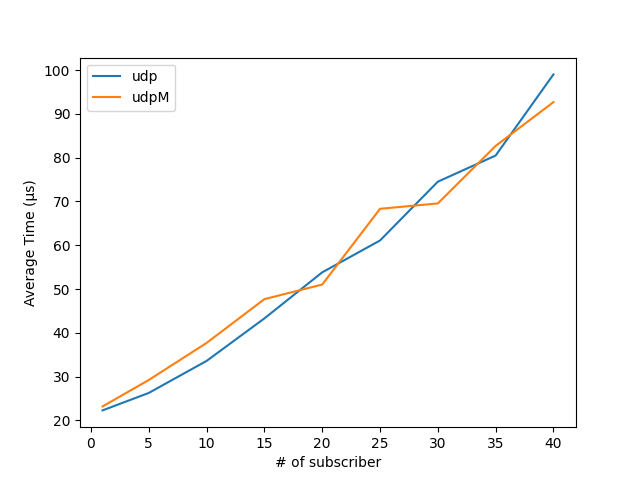
\includegraphics[width=\textwidth]{./results/test3_udpvsudpM.png} 
        \caption{} %TODO: caption
        \label{}
\end{figure}

Da questo si può concludere che sia il publisher che subscriber risentono della presenza di molteplici ascoltatori su un topic. Questo problema è facilmente risolvibile lato publisher utilizzando protocolli che si basano su multicast. 


\section{Primo messaggio}
E' stato notato in tutte le comunicazioni effettuate un ritardo, di un ordine di grandezza superiore, che riguarda esclusivamente il primo messaggio. Tuttavia, non è stato chiarito il motivo di questo \gls{overhead}, presente anche in comunicazioni locali\footnote{comunicazioni effettuati in localhost o in shared memory}. Anche se non dimostrato una delle possibili motivazioni potrebbe essere la necessità di allocare memoria durante la prima fase di comunicazione, da entrambi gli attori (potenzialmente amplificato nel caso \ref{fig:rtt_uml}). 
\begin{figure}[H]
    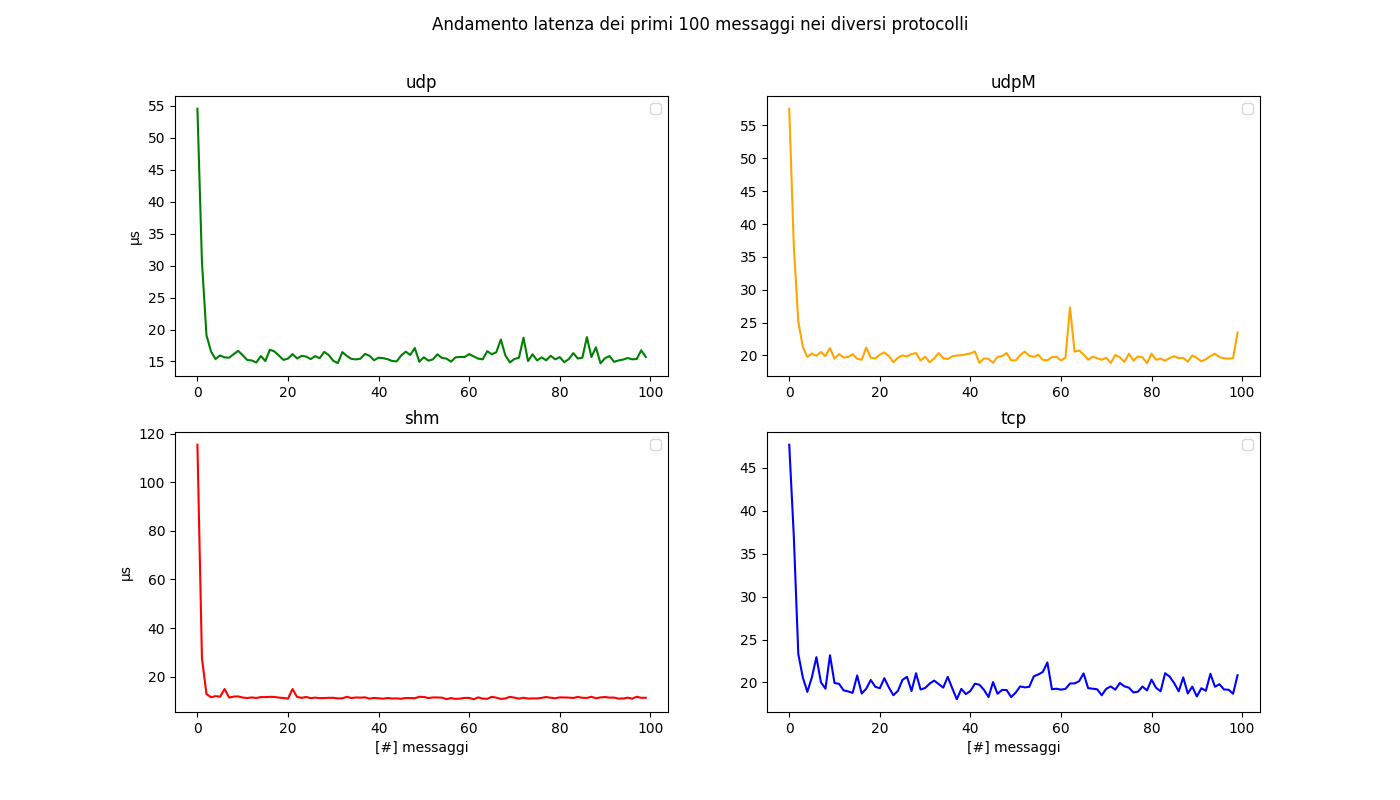
\includegraphics[width=\textwidth]{./results/errortest.png} 
    \caption{} %TODO: caption
    \label{}
\end{figure}
Data la complessità necessaria per andare così a fondo nel problema, non è stato approfondito ulteriormente.

\section{test-1}
I risultati che sono stati trovati forniscono importanti informazioni, %TODO: to finish

\begin{figure}[H]
    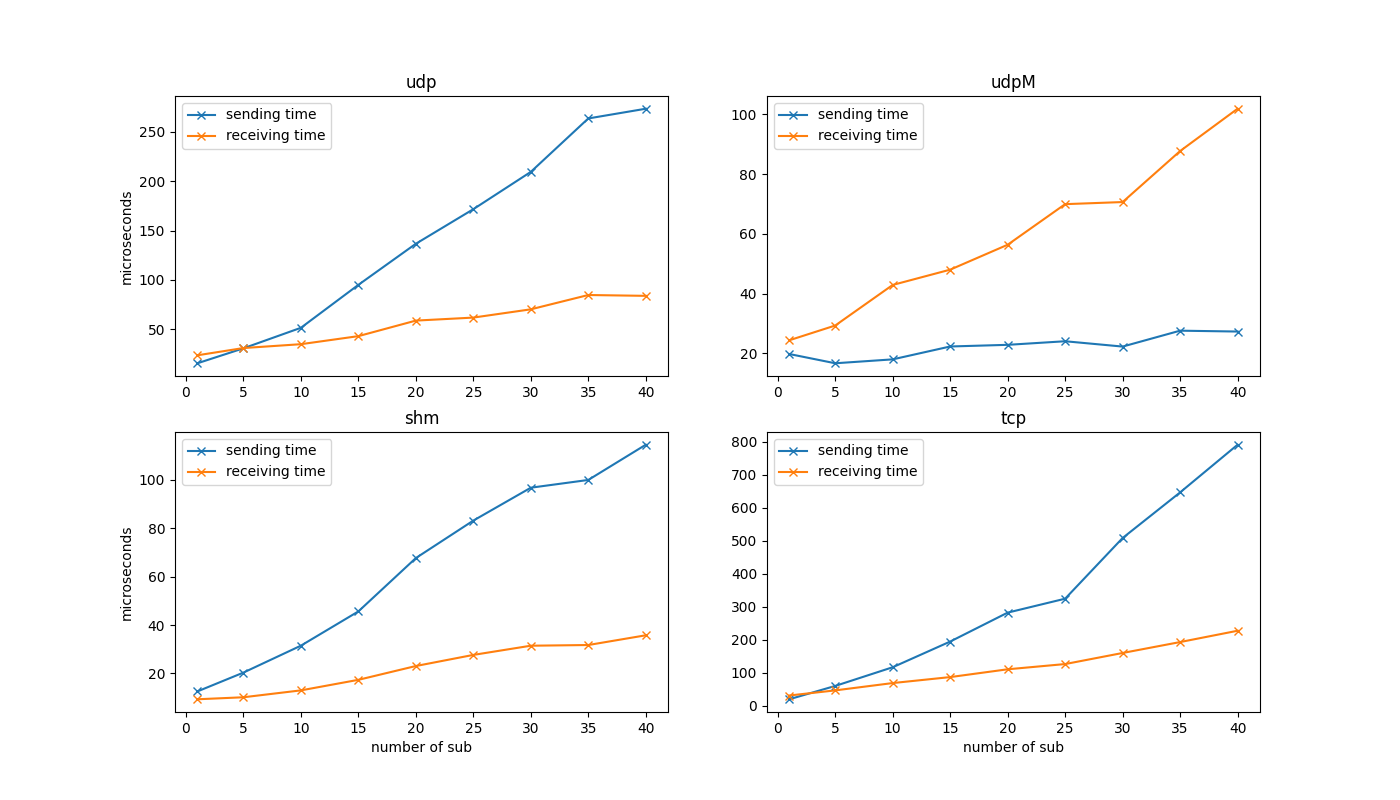
\includegraphics[width=\textwidth]{./results/test3_different_protocol_send_receive.png} 
        \caption{differenza tra solo publish e publish-subscribe per ogni protocollo}
        \label{fig:test3_different_protocols}
\end{figure}

\begin{figure}[H]
    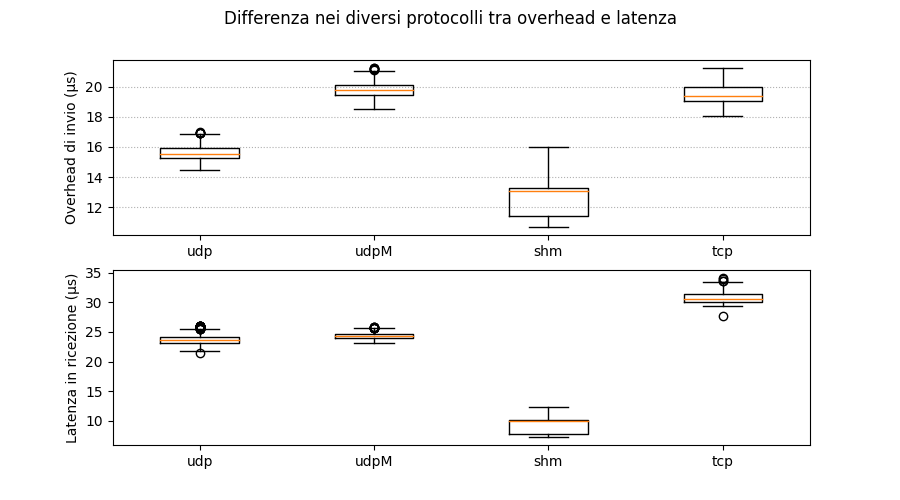
\includegraphics[width=\textwidth]{./results/test1_box_sr_1p1s.png} 
        \caption{diagramma a scatola nei vari protocolli di comunicazione}
        \label{fig:test1sdbox}
\end{figure}

\begin{figure}[H]
    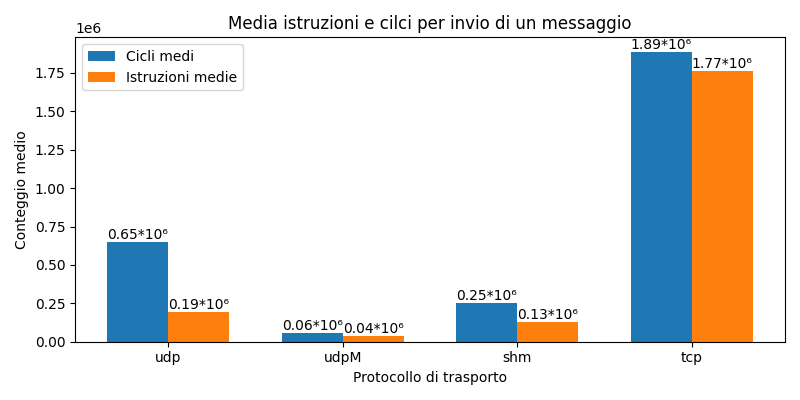
\includegraphics[width=\textwidth]{./results/test1_cyclinstr.png} 
        \caption{Conteggio cicli e istruzioni per ogni protocollo}
        \label{fig:test3_different_protocols}
\end{figure}

\section{test-2}

Nei test effettuati con domini, topic e partizioni, non sono state notate differenze degne di nota in termini di performance (cicli e istruzioni) nell'usare uno strumento piuttosto che un altro. %TODO ADD GRAPH

\section{test-3}

\begin{figure}[H]
    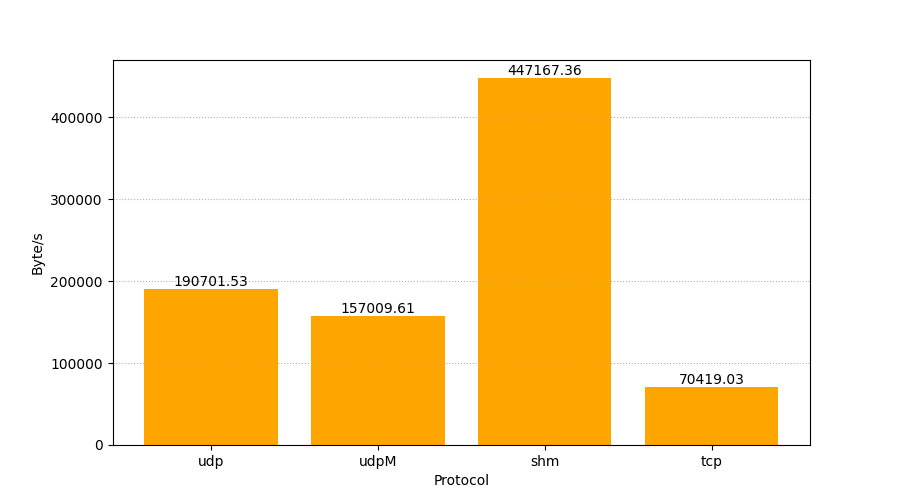
\includegraphics[width=\textwidth]{./results/test3_throughput.png} 
        \caption{} %TODO: caption
        \label{}
\end{figure}

\begin{figure}[H]
    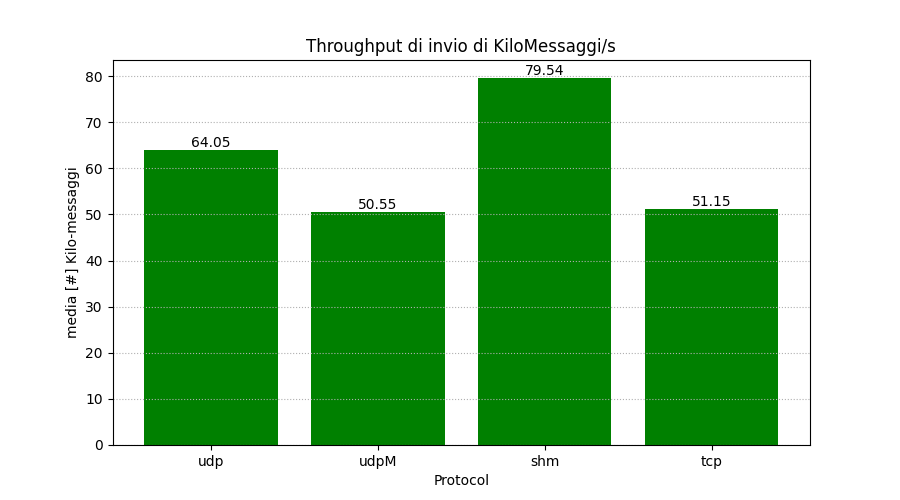
\includegraphics[width=\textwidth]{./results/test3_throughput_m.png} 
        \caption{} %TODO: caption
        \label{}
\end{figure}


\begin{figure}[H]
    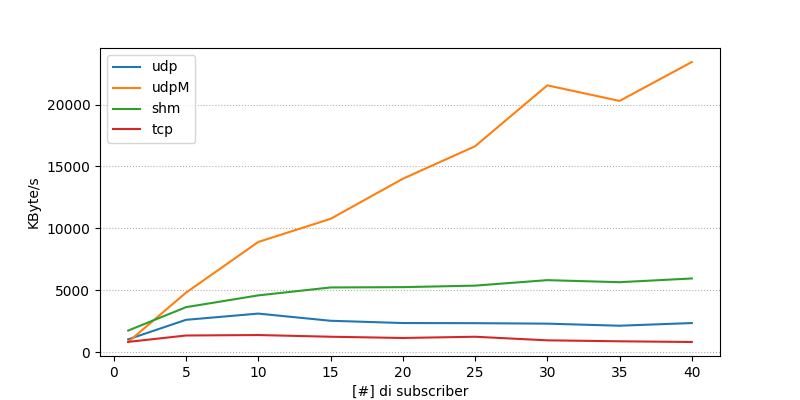
\includegraphics[width=\textwidth]{./results/test3_graph_throughput.png} 
    \caption{} %TODO: caption
    \label{}
\end{figure}






\section{Modello}